

\chapter{Introduciton to Multirate Signal Processing}

\section{Donwsampling}

What happen to the time frequency index when doing downsampling.\\

From frequency sampling and DFT computations, we know that when computing a frequency bin numerically, the frequency step is $\displaystyle\frac{2 \pi}{N}$, where $N$ is the total number of samples (the length of the discrete time signal or the sampled signal).\\

So we have the relation:

\begin{equation}
f \, \times \, t \, \leftrightarrow \, n \, \times \,  \displaystyle\frac{k}{N}
\end{equation}

where:

\begin{itemize}
    \item $f$ and $t$ are some indexes for continuous frequency and time 
    
    \item $n$: discrete time index
    
    \item $k$: discrete frequency index
\end{itemize}

When we downsample by a factor of $D$, the relation between the indices is:
\begin{equation}
\displaystyle\frac{k \, n}{N} \leftrightarrow   \displaystyle\frac{k \, n}{N/D}
\end{equation}

Also recall that $F_s \geq \, 2 \, f$, but a more equivalent common form is $f \leq \, \displaystyle\frac{F_s}{2}$, which mean the analog baseband frequency is captures between the range 0 to $\displaystyle\frac{F_s}{2}$. So we can say:

\begin{equation}
  F_s \geq \, 2 \, f \, \equiv  f \leq \, \displaystyle\frac{F_s}{2} 
\end{equation}

\newpage
\underline{What happen when we downsample?}\\

If we begin with a signal with a sampling rate $F_s$, where the CTFT spectrum contains $N$ point ($N$ is the total number of samples with a sampling period $T_s \, = \, \displaystyle\frac{1}{F_s}$).\\

Let's take an example of a sin wave, where its CTFT spectrum is shown in \autoref{fig:Multirate:sin_wave_CTFT}.


\begin{figure}[h]
\centering
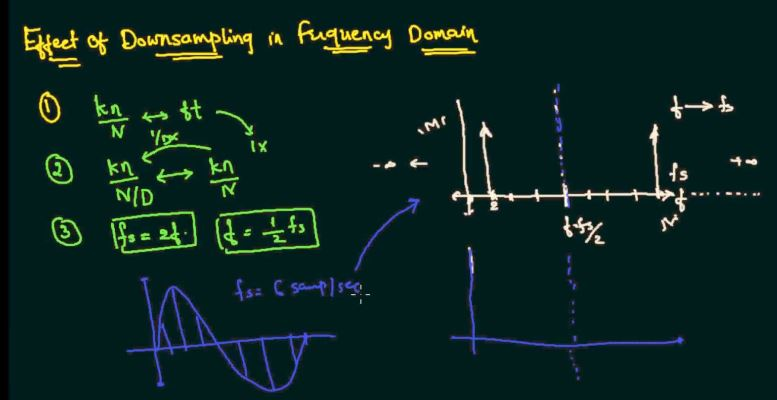
\includegraphics[scale = 0.5]{Figures/Multirate/sin_wave_CTFT}
\caption{Sine Wave CTFT Spectrum}
\label{fig:Multirate:sin_wave_CTFT}
\end{figure}

The original $F_s \, = \, 6 Hz$, that is 6 sample per cycle (this in the time domain), and the DFT spectrum for the CTFT contains $N \, = \, 6$ frequency fundamental points (for a window duration of 1s let's say).\\

\newpage
If we downsample and let the new $F_s$ 3 Hz, that is $F_s^D \, = \, 3$ Hz, we will have:

\begin{itemize}
    \item 3 samples per cycle (period) instead of 3 $\leftrightarrow$ time domain effect
    
    \item Frequency domain effect (see \autoref{fig:Multirate:sin_wave_CTFT_downsample}):
    
        \begin{itemize}
        
        \item Folding line $\displaystyle\frac{F_s}{2}$ will get closer
        
        \item Frequency points indices will also get lost because $N$ is reduced , but the frequency index 2 remain fix $\leftrightarrow$ so the spectrum get preserved
        \end{itemize}
    
\end{itemize}

\begin{figure}[h]
\centering
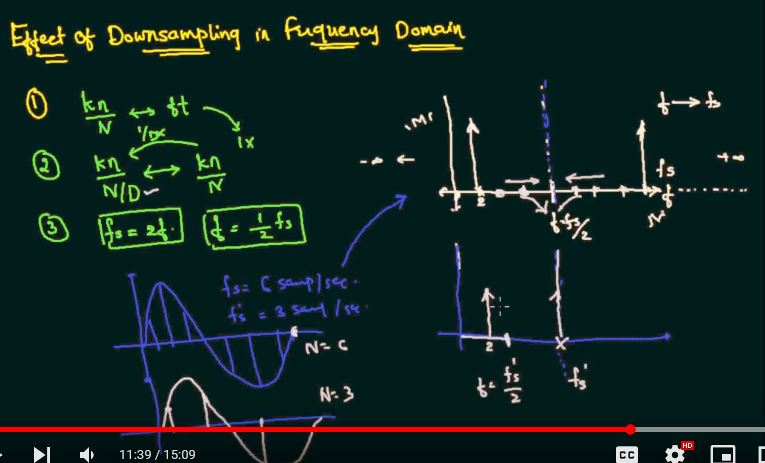
\includegraphics[scale = 0.5]{Figures/Multirate/sin_wave_CTFT_downsample}
\caption{Sine Wave CTFT Spectrum}
\label{fig:Multirate:sin_wave_CTFT}
\end{figure}

Important note: if we do dowsanmpling, it is not necessarily that aliaising get occurred.\\

A more general example for a bandlimited signal is shown in \autoref{fig:Multirate:CTFT_bandlimited_downsample} 

\begin{figure}[h]
\centering
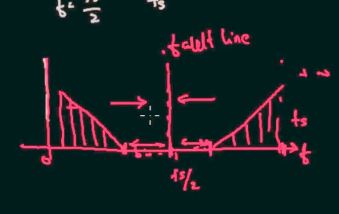
\includegraphics[scale = 0.8]{Figures/Multirate/CTFT_bandlimited_downsample}
\caption{Sine Wave CTFT Spectrum}
\label{fig:Multirate:CTFT_bandlimited_downsample}
\end{figure}

When we downsample, the folding line $\displaystyle\frac{F_s}{2}$ will get closer (move to the left). As long as the new folding line $\displaystyle\frac{F^D_s}{2} \ \, > \, f_{max}$, the signal spectrum is preserved and no aliasing occur.

\subsection{Example: Downsampling with no aliasing}


\todo{dowsampling with no aliasing}: to redo with a sinc example.

We take a numerical example to illustrate downsampling.\\

First we generate a bandlimited signal with a bandwidth of 100 Hz, generated using the \verb|fir2| command.\\

The $\omega_{\text{pass}} \, = \, 0.25 \pi$, and the correspondent analog frequency $f_{\text{pass}} \, = \, \omega_{\text{pass}} \, \times \, F_s \, \times \, \frac{1}{2 \pi} \, = \, 100 Hz$.\\


The initial sampling rate $F_s^{\text{init}} \, = \, 800 Hz$, and we downsample by a factor 4, so the new sampling rate $F_s^{D} \, = \, \displaystyle\frac{F_s^{\text{init}}}{D} \, = \, \displaystyle\frac{800}{4} \, = \, 200 $ Hz.\\

Notice that new folding line now is $ \displaystyle\frac{F_s^{D}}{2} \, = \, 200 > \, 100$, where the 100 is the bandwidth of the signal, so no aliasing will occur and the bandwidth will still the same.

\newpage
\section{Downsampling with Aliasing}

\underline{Note:} this section contains many simulations and explanation, and since they have allot of details and contain many points, I decided to make it as a section instead of a subsection.\\ 


\subsection{Example 1: Aliased Sin and Cos}
\label{Sub:Downsampling_Aliasing}

\underline{Ref:} chapter 11 in \cite{book_Li_Tan_dsp_fundamentals_and_app}.\\

We take 1 cos and sin signal as the following:

\begin{equation}
    x(t) \, = \, 5 \sin(2 \, \pi 10^3 \, t ) \, + \, \cos(2 \, \pi \, 2.5 \, \times \, 10^3 \, t)
\end{equation}

\begin{itemize}
    \item Frequency of each component is at 1 KHz and 2.5 KHz
    
    \item $F_s \, = \, 8$ KHz
\end{itemize}

For $F_s \, = \, 8$ KHz, the folding frequency is at $\displaystyle\frac{F_s}{2} \, = \, 4$ KHz $> 2.5 $KHz, so no aliasing occur.\\

Let's say we downsample by a factor $D \, = \, 2$, so we will have:

\begin{itemize}
    \item $F_{s_D} \, = \, \displaystyle\frac{F_s^{\text{orig}}}{D} \, = \, \displaystyle\frac{8000}{2} \, = \, 4$ KHz
    
    
    \item The new folding frequency will be $\displaystyle\frac{4000}{2} \, = \, 2000$ Hz  $ < \, 2500$ Hz
    
\end{itemize}

In this case, the new folding frequency is smaller then the bigger frequency component in $x(t)$, so aliasing will occur in the reconstructed signal.\\

\newpage
\underline{Computation of the aliased frequency:}\\

The alias frequency will be smaller then the new sampling rate $F_{sD} \, = \, 4$ KHz, and it can be computed as:

\begin{equation}
    \begin{array}{rcl}
        f_{\text{alias}} &=& \, F_{sD} \, - \,  f_{\text{max}}   \\
         &=& 4 \text{ KHz} \, - \, 2.5 \text{ KHz} \\
         &=& \, 1.5 \text{ KHz}
    \end{array}
\end{equation}


\begin{figure}[h]
\centering
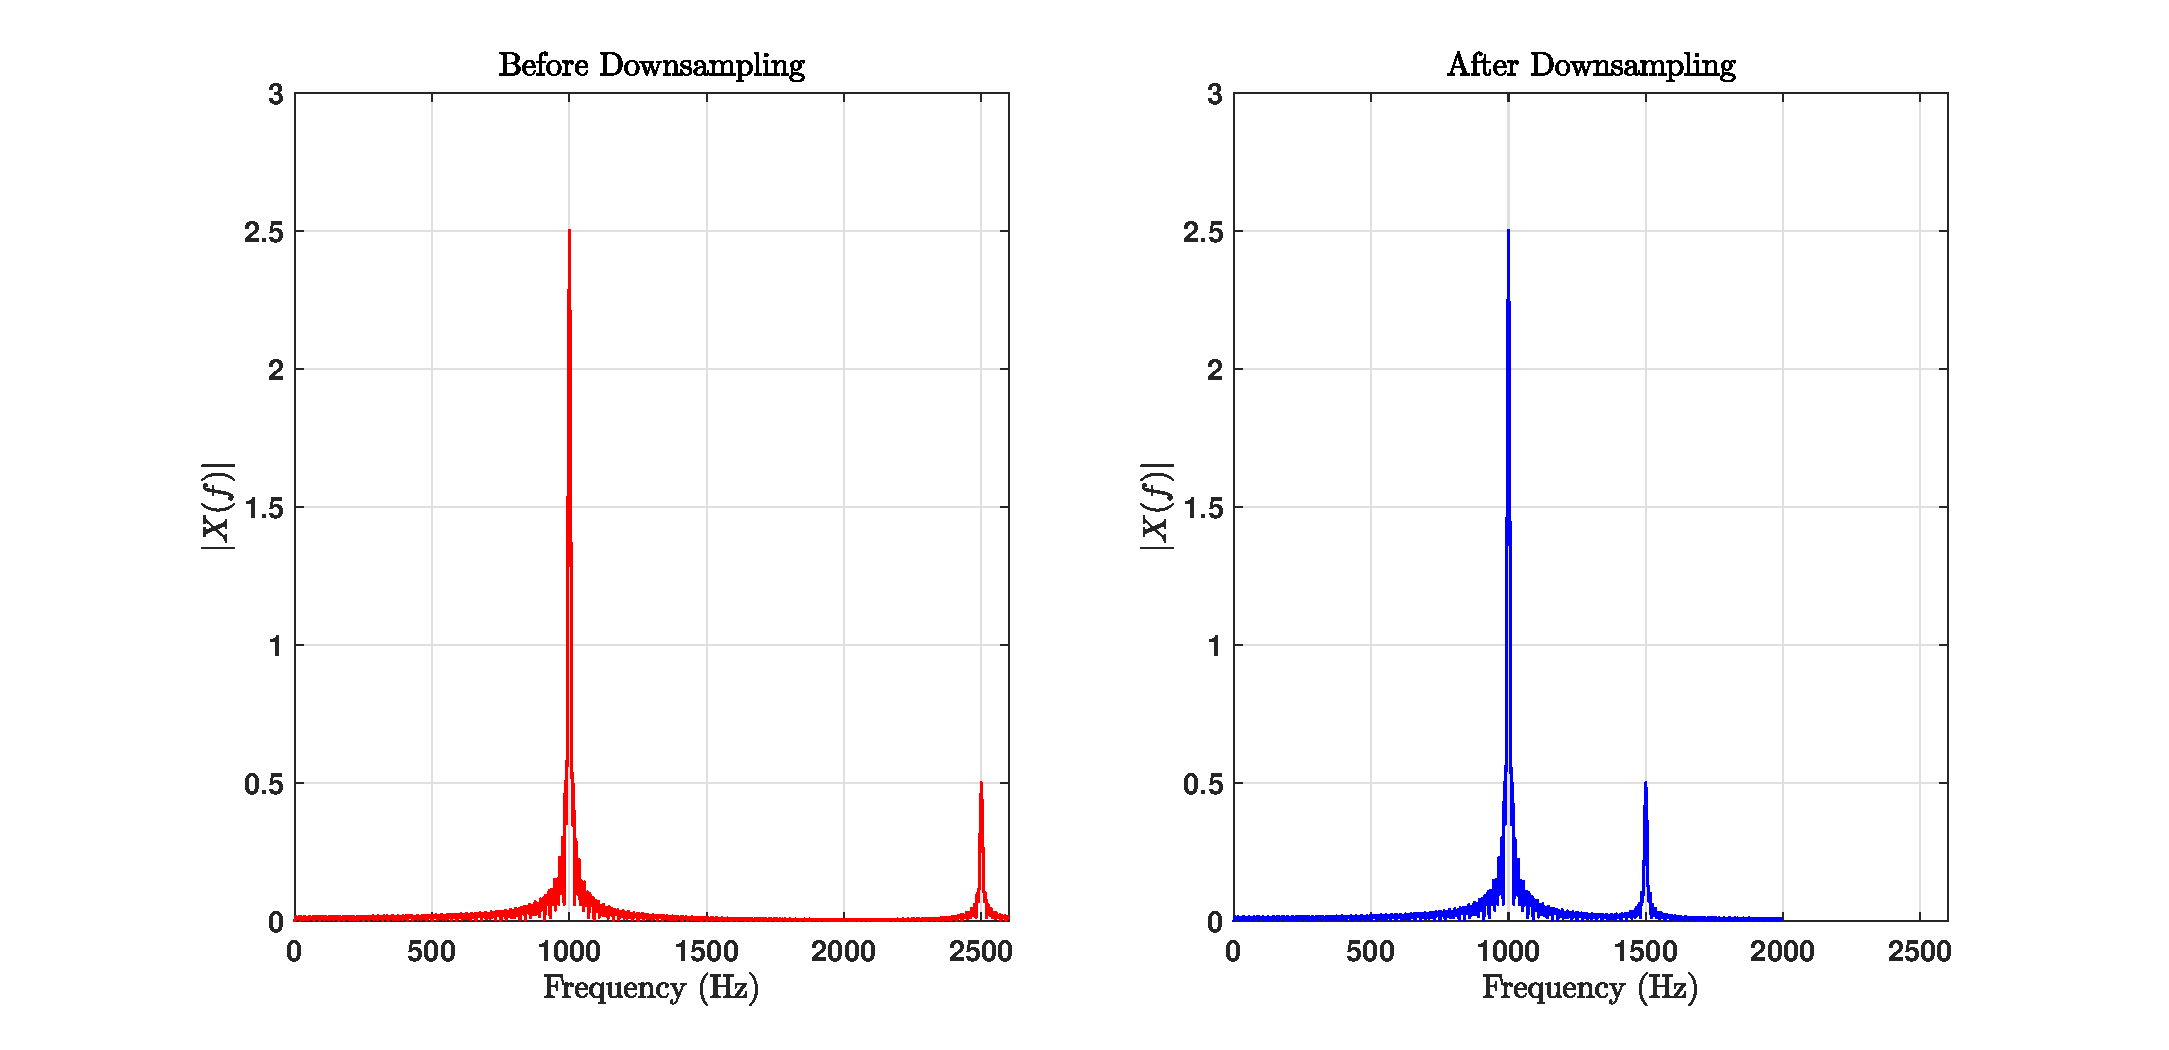
\includegraphics[scale = 0.5]{Figures/Multirate/a_Aliasing_Changing_Fs}
\caption{Sine Wave CTFT Spectrum}
\label{fig:Multirate:a_Aliasing_Changing_Fs}
\end{figure}


\underline{Example 2:}\\

In example 1, we have illustrated the aliasing by keeping the frequency of the signal constant and changing $F_s$, but also we can illustrate the aliasing by changing the frequency of the signal (like we have some signal generator with variable input frequencies) and keep $F_s$ constant.\\

\newpage
\subsection{Example 3: Aliasing with a full bandlimited signal}

Example 1 in \ref{Sub:Downsampling_Aliasing} focus on visualizing the aliasing with only sin (or cos) signals, or the sum of many sin.\\

The sin spectrum consist only of 1 peak at the location of frequency of the sin. Now we try to simulate the aliasing with signals where the spectrum extend from $0 \, \rightarrow \, B$[Hz].\\

\underline{Note of vocabulary:} by \textit{full bandlimited signal}, I mean that the amplitude spectrum is present over all the bandwidth $B$, not only over 1 frequency component like the sin or cos signals

So as example, we take the sinc signal.\\


\newpage
\subsubsection{Flow of the explanation}


\begin{itemize}

\item When I was try to debug the problem, I deiced to start with other test signal then sin or cos $\leftrightarrow$ signals that have only 1 frequency components


\item As a choice I took a sinc signal (See section 3.2.3 in \cite{sampling_beyond_band_limited_systems}):

\begin{equation}
  \text{sinc}\left(\,  \displaystyle\frac{t}{T}  \, \right) \, \leftrightarrow \, X(\Omega) \, = \, T \quad \text{ for } \displaystyle\frac{-\pi}{T} \, \leq  \, \Omega \, \leq \,  \displaystyle\frac{\pi}{T}  
\end{equation}

\item Parameters in simulation:

\begin{itemize}
    \item $B \, = \, 10$ Hz

    \item A \textit{big time window} from $-50 \rightarrow \, 50$ s
    
    \begin{itemize}
        \item So when simulating aliasing phenomena, I ensure that my source of error is only in low $F_s$ and not in a small time window
        
        \item Also I start before $t \, = \, 0$, so I don't assume causality of signal for now
        
    \end{itemize}
    
\end{itemize}

\item \underline{Result of Input Analog Signal:}

\begin{figure}[h]
\centering
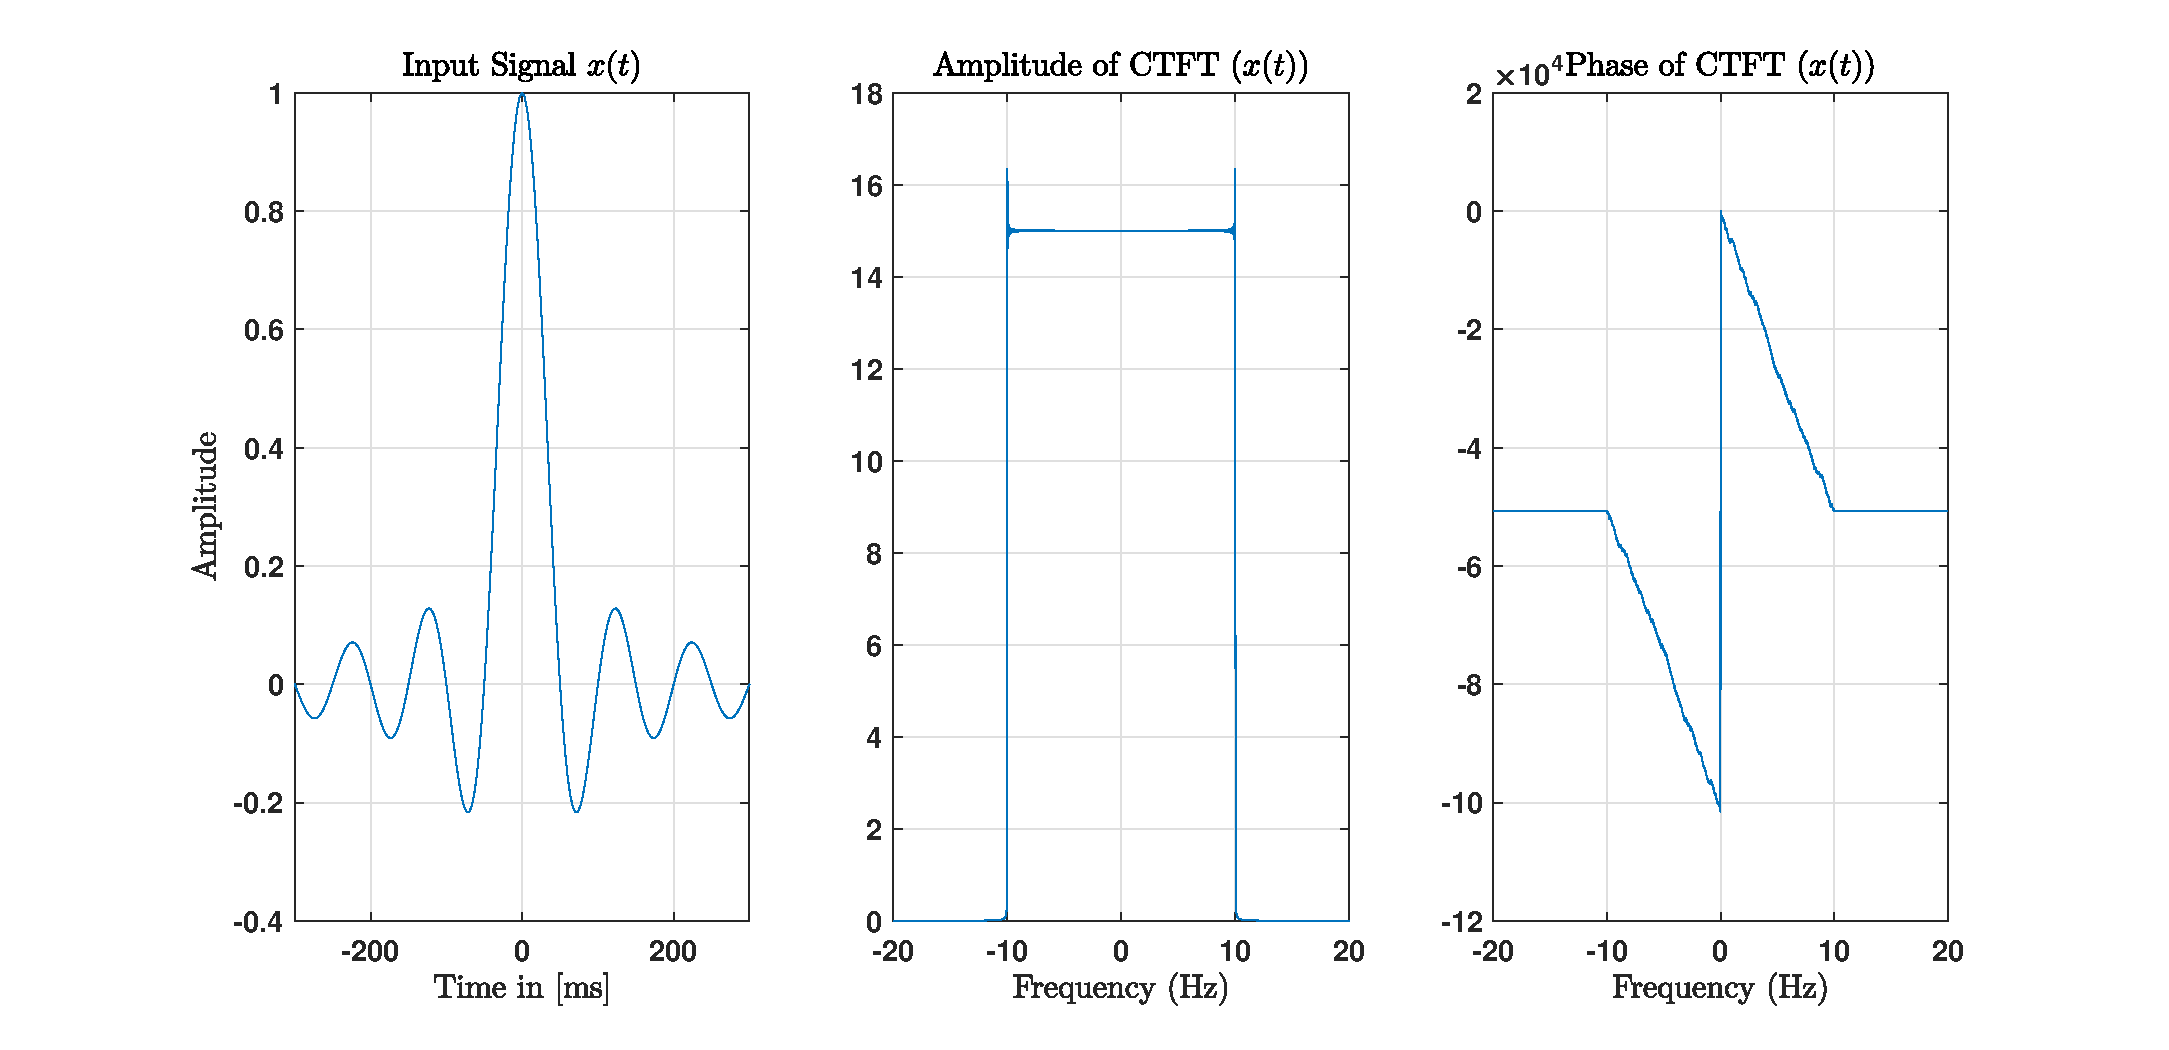
\includegraphics[scale = 0.5]{Figures/Sim_dowsampling_upsampling/Sinc_Input_Analog_B_10_Hz}
\caption{Input Analog Sinc signal}
\label{fig:Sim_dowsampling_upsampling:Sinc_Input_Analog_B_10_Hz}
\end{figure}


\begin{itemize}
    \item For analog simulation, I use oversampling to create a fine grid of analog time where $F_{s_{\text{analog}}} \,  = \, \text{oversampling } \times \, B$.
    
    In the code I took the oversampling $= \, 30 \rightarrow \, F_{s_{\text{analog}}} \, = \,300$ Hz
    
    \item For now I don't use any postprocessing (divide by the number of samples for example in a sin or a cos signal) for the FFT command to adjust the magnitude or the phase.
    
    I focus for now that the shape of the magnitude spectrum is correct with a correct bandwidth
    
   
\end{itemize}


\item To simulate any other $F_s$, I use \textit{integer} dowsampling operation where $D \, = \,\displaystyle\frac{F_{s_{\text{original}}}}{F_{s{\text{target}}}} \,  \in \mathbb{N} $ such that $ F_{s{\text{target}}}  \, < \, F_{s_{\text{original}}}$

\item To ensure my dowsampling operation is correct, I choose 2 $ F_{s{\text{target}}} \, = \, [60 \, , \, 30]$ Hz

\begin{itemize}
    \item Both $F_{s{\text{target}}} \, > \, F_{\text{Nyquist}} \, = \, 2 \, \times \, F_{H} \, = \, 20 $ Hz $\rightarrow$ no aliasing occur, and we will be able to do reconstruction 
\end{itemize}


\underline{Results:} CTFT Amplitude Spectrum

\begin{figure}[h]
\centering
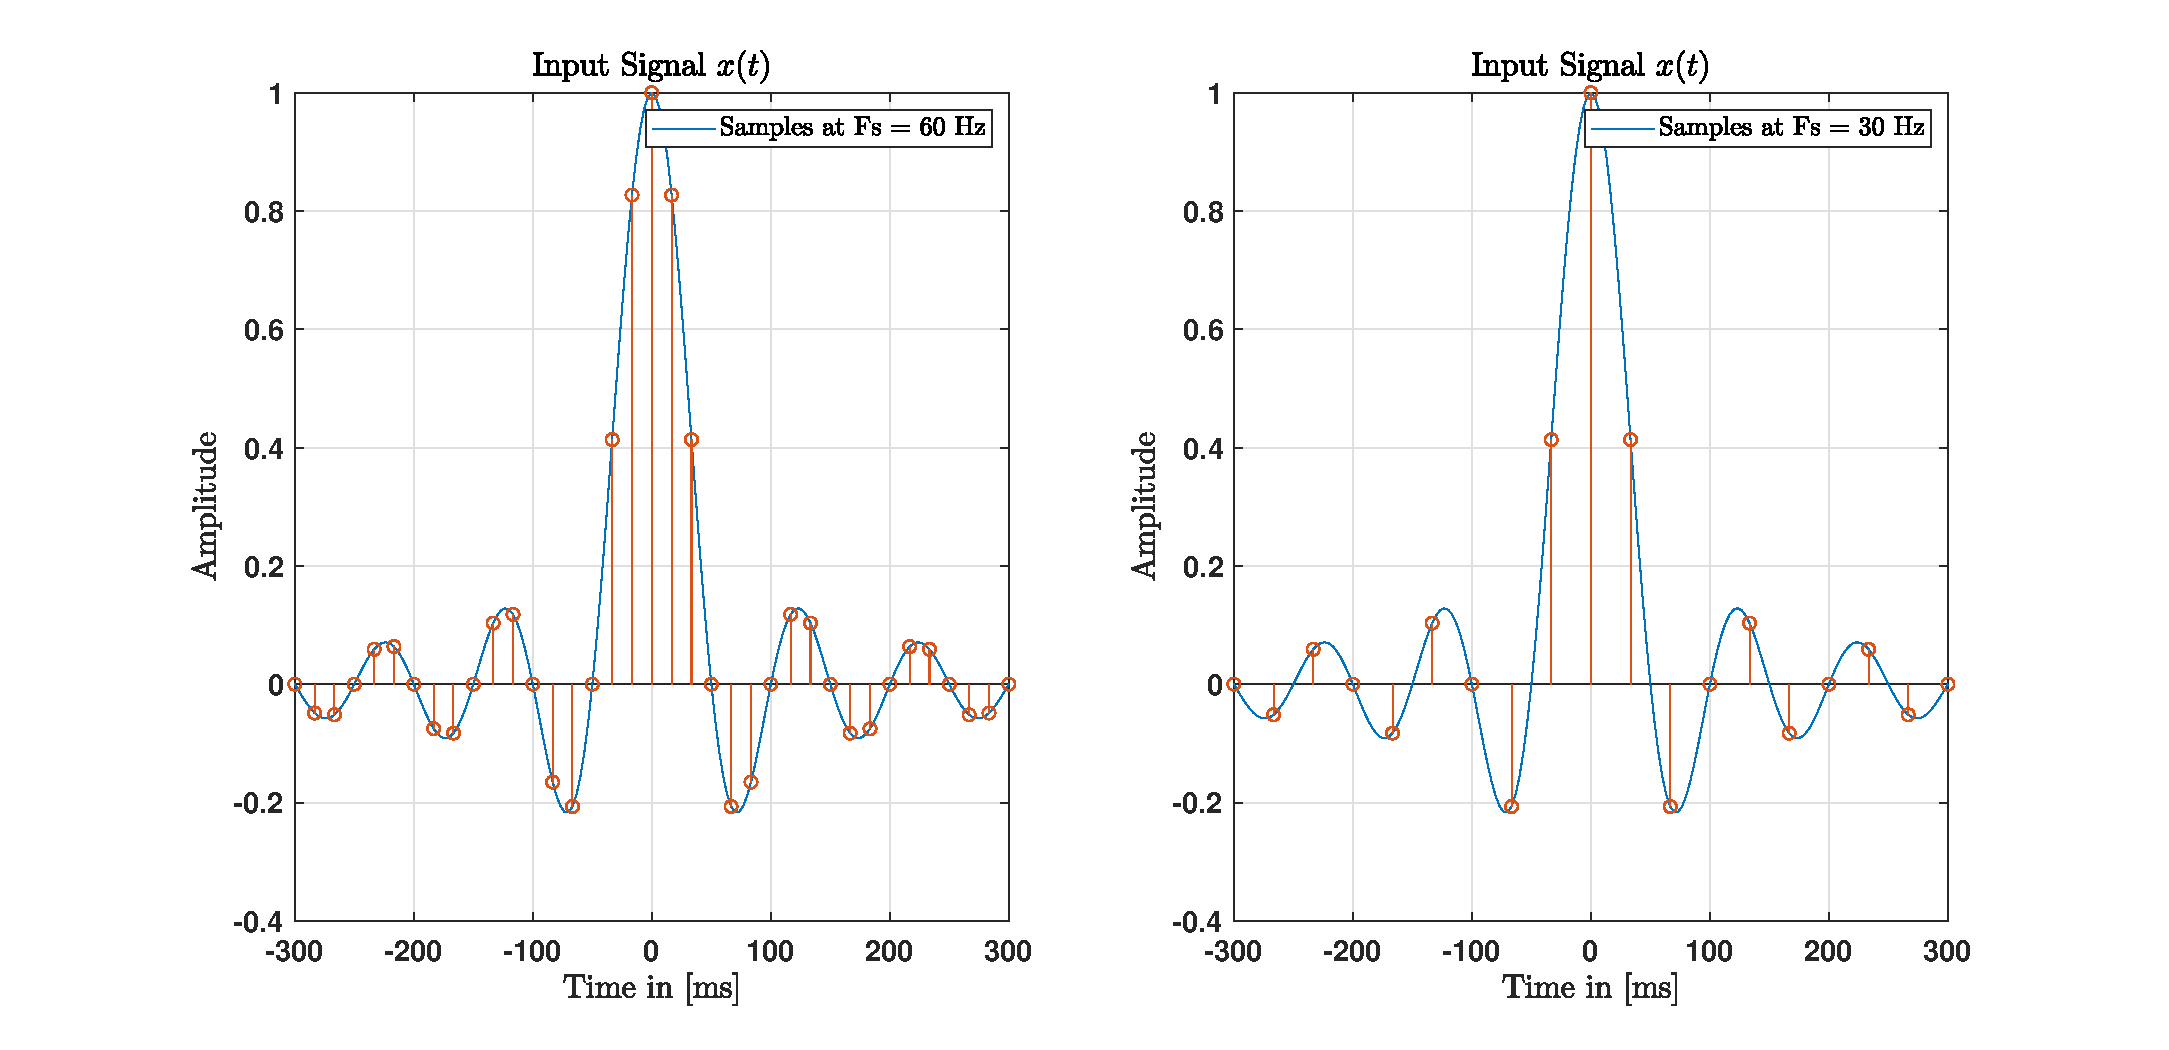
\includegraphics[scale = 0.4]{Figures/Sim_dowsampling_upsampling/downsample_sinc_Fs_30_and_60_Hz}
\caption{Ideal Reconstruction}
\label{fig:Sim_dowsampling_upsampling:downsample_sinc_Fs_30_and_60_Hz}
\end{figure}

\newpage

\begin{figure}[h]
\centering
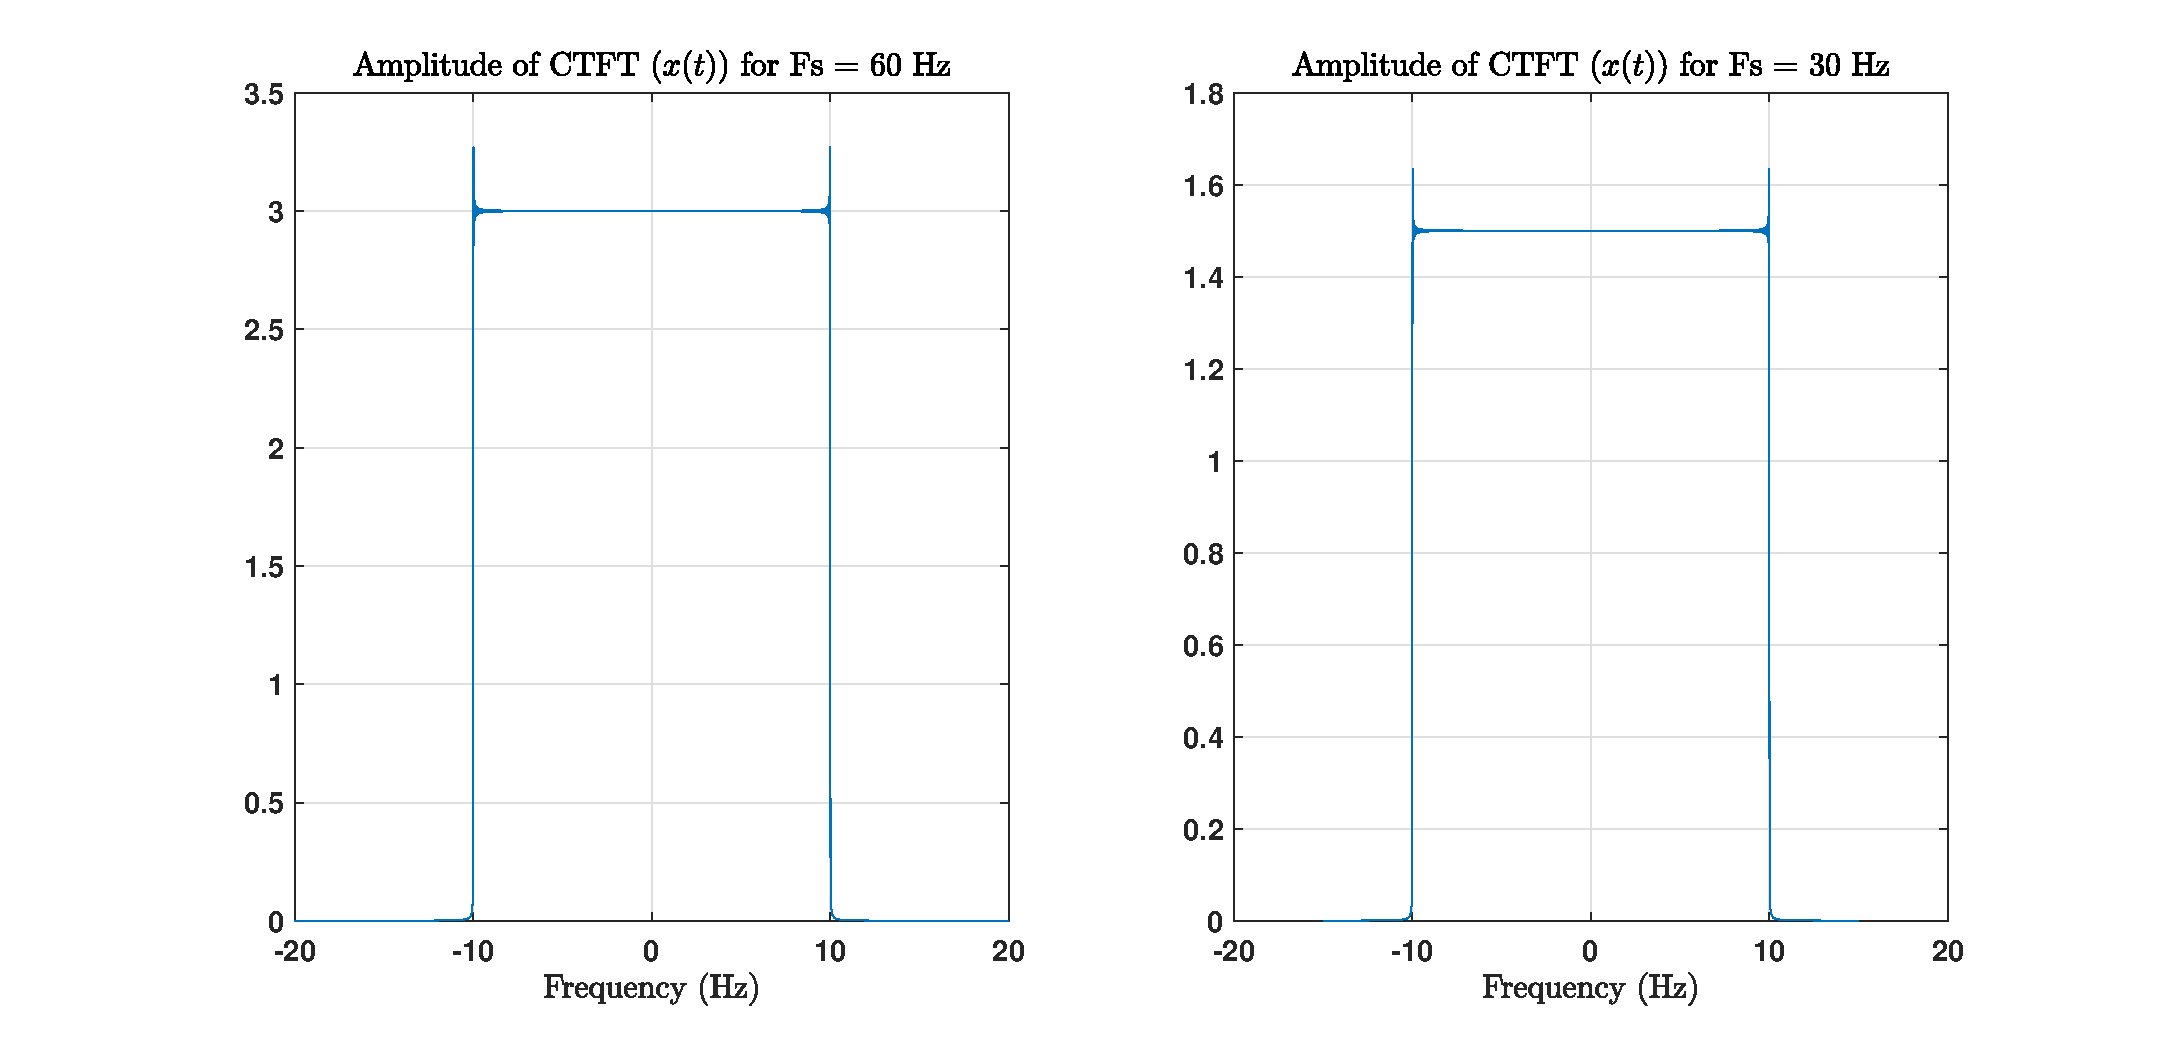
\includegraphics[scale = 0.4]{Figures/Sim_dowsampling_upsampling/CTFT_Amp_Sinc_B_10_Fs_30_60}
\caption{CTFT Amplitude Spectrum}
\label{fig:Sim_dowsampling_upsampling:CTFT_Amp_Sinc_B_10_Fs_30_60}
\end{figure}


\begin{figure}[h]
\centering
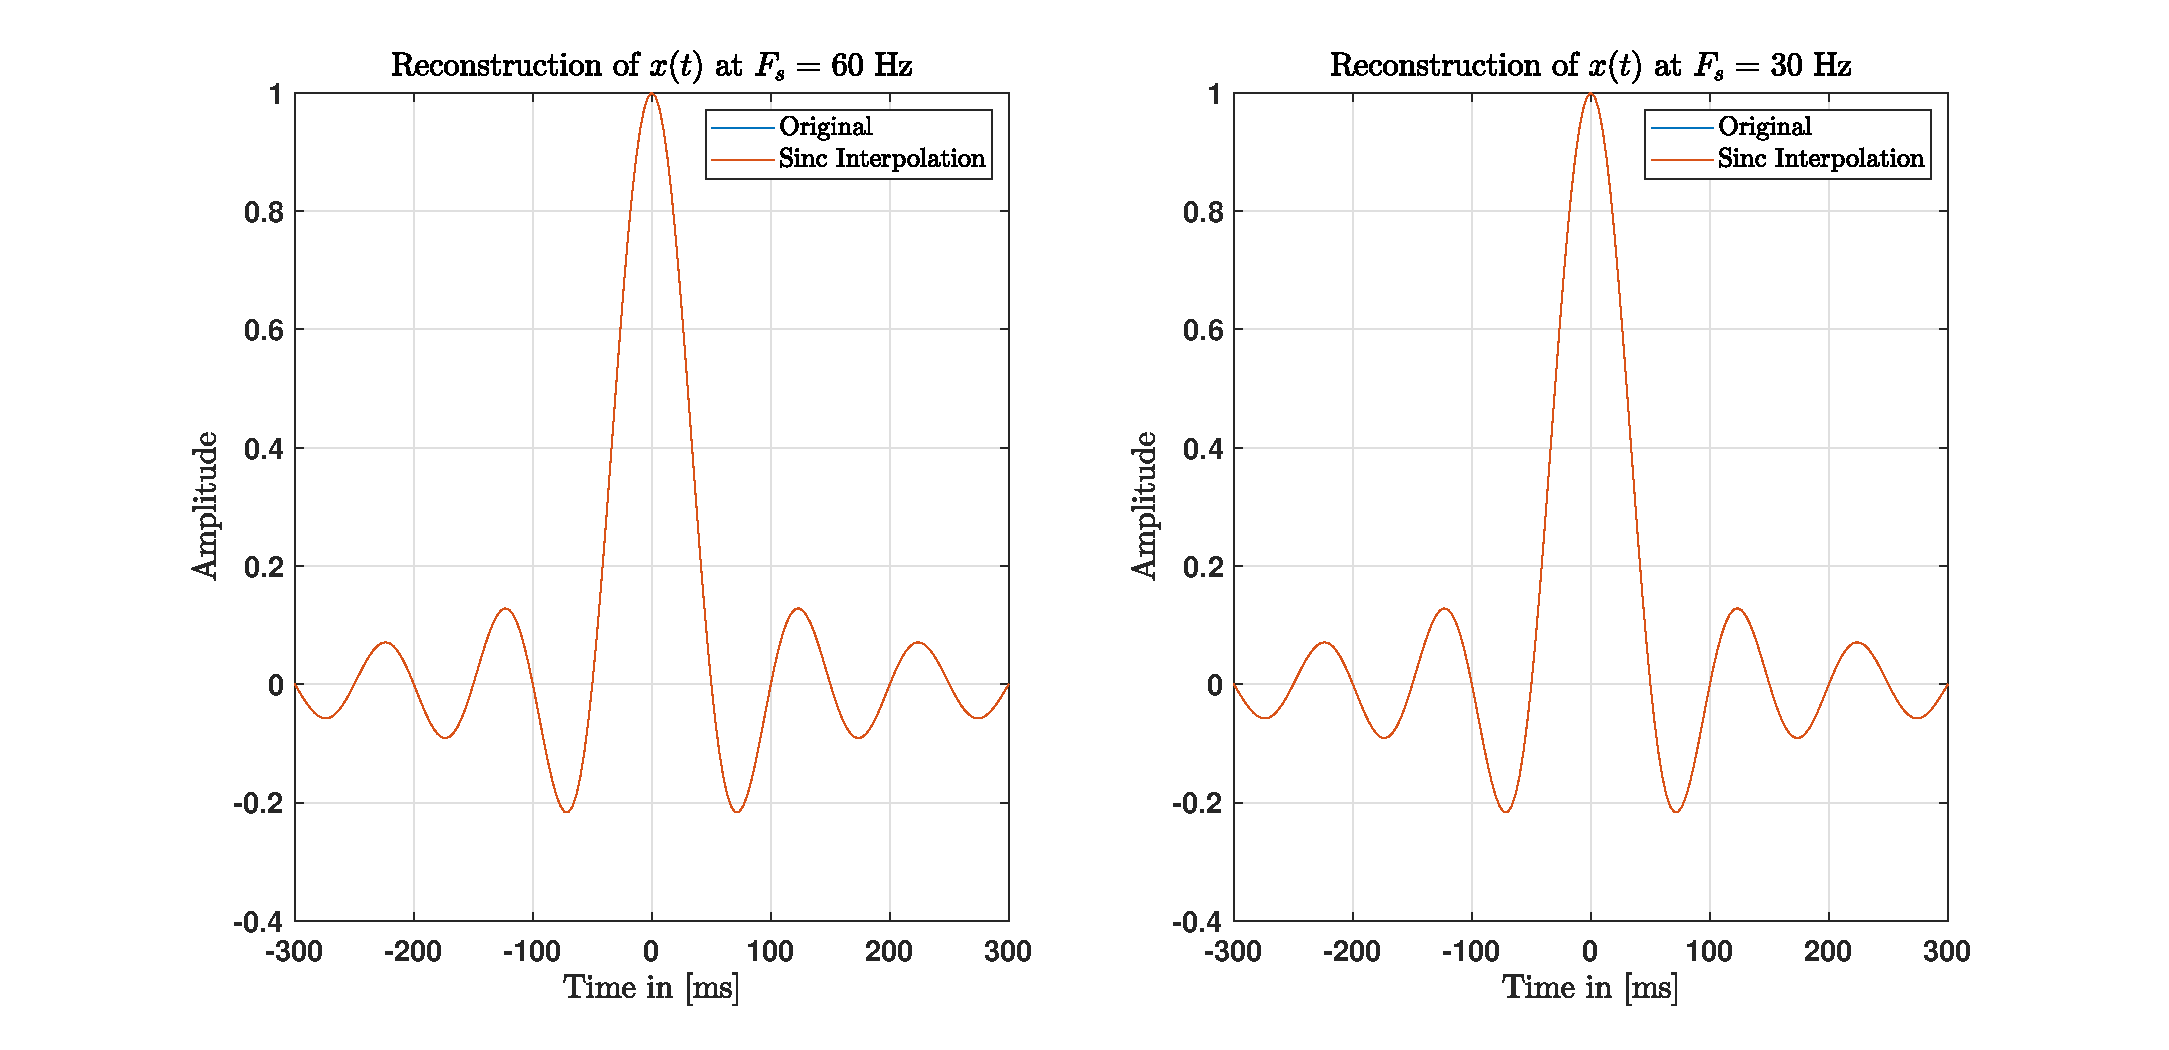
\includegraphics[scale = 0.4]{Figures/Sim_dowsampling_upsampling/Interpolation_Sinc_Fs_30_60_Hz_B_10_Hz}
\caption{Ideal Reconstruction}
\label{fig:Sim_dowsampling_upsampling:Interpolation_Sinc_Fs_30_60_Hz_B_10_Hz}
\end{figure}


\newpage

\item Now I decide to choose a $F_s \, < \, F_{\text{Nyquist}}$

\begin{itemize}
    \item From theory, when we drop $F_s$ below $F_{\text{Nyquist}} \,  \equiv \, \Omega_s \, < \, 2\, \Omega_H$, \textit{aliasing} should occur
\end{itemize}

\begin{figure}[h]
\centering
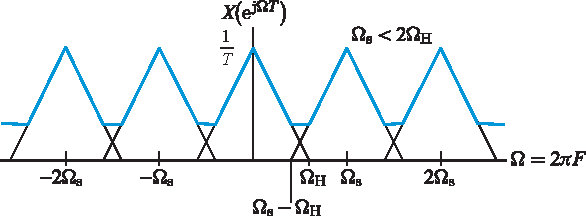
\includegraphics[scale = 0.9]{Figures/Sim_dowsampling_upsampling/aliasing_illustration}
\caption{Aliasing when $\Omega_s \, < \, 2\, \Omega_H$ \cite{DSP_DimitrisManolakis}}
\label{fig:Sim_dowsampling_upsampling:aliasing_illustration}
\end{figure}

\begin{itemize}
    
    \item From \autoref{fig:Sim_dowsampling_upsampling:aliasing_illustration}, we can say that:
    
    \begin{enumerate}
        \item Part of the spectrum is preserved and the other part which \textit{don't respect Nyquist theorem} is distorted
        
        \item But the signal spectrum still at $\Omega_H$ but distorted (I will clarify this point later in simulation)
    \end{enumerate}

    \item I tried to take $F_{s_{\text{ch}}} \, = \, 15$ Hz
    
    \item Result:
    
\end{itemize}

\begin{figure}[h]
\centering
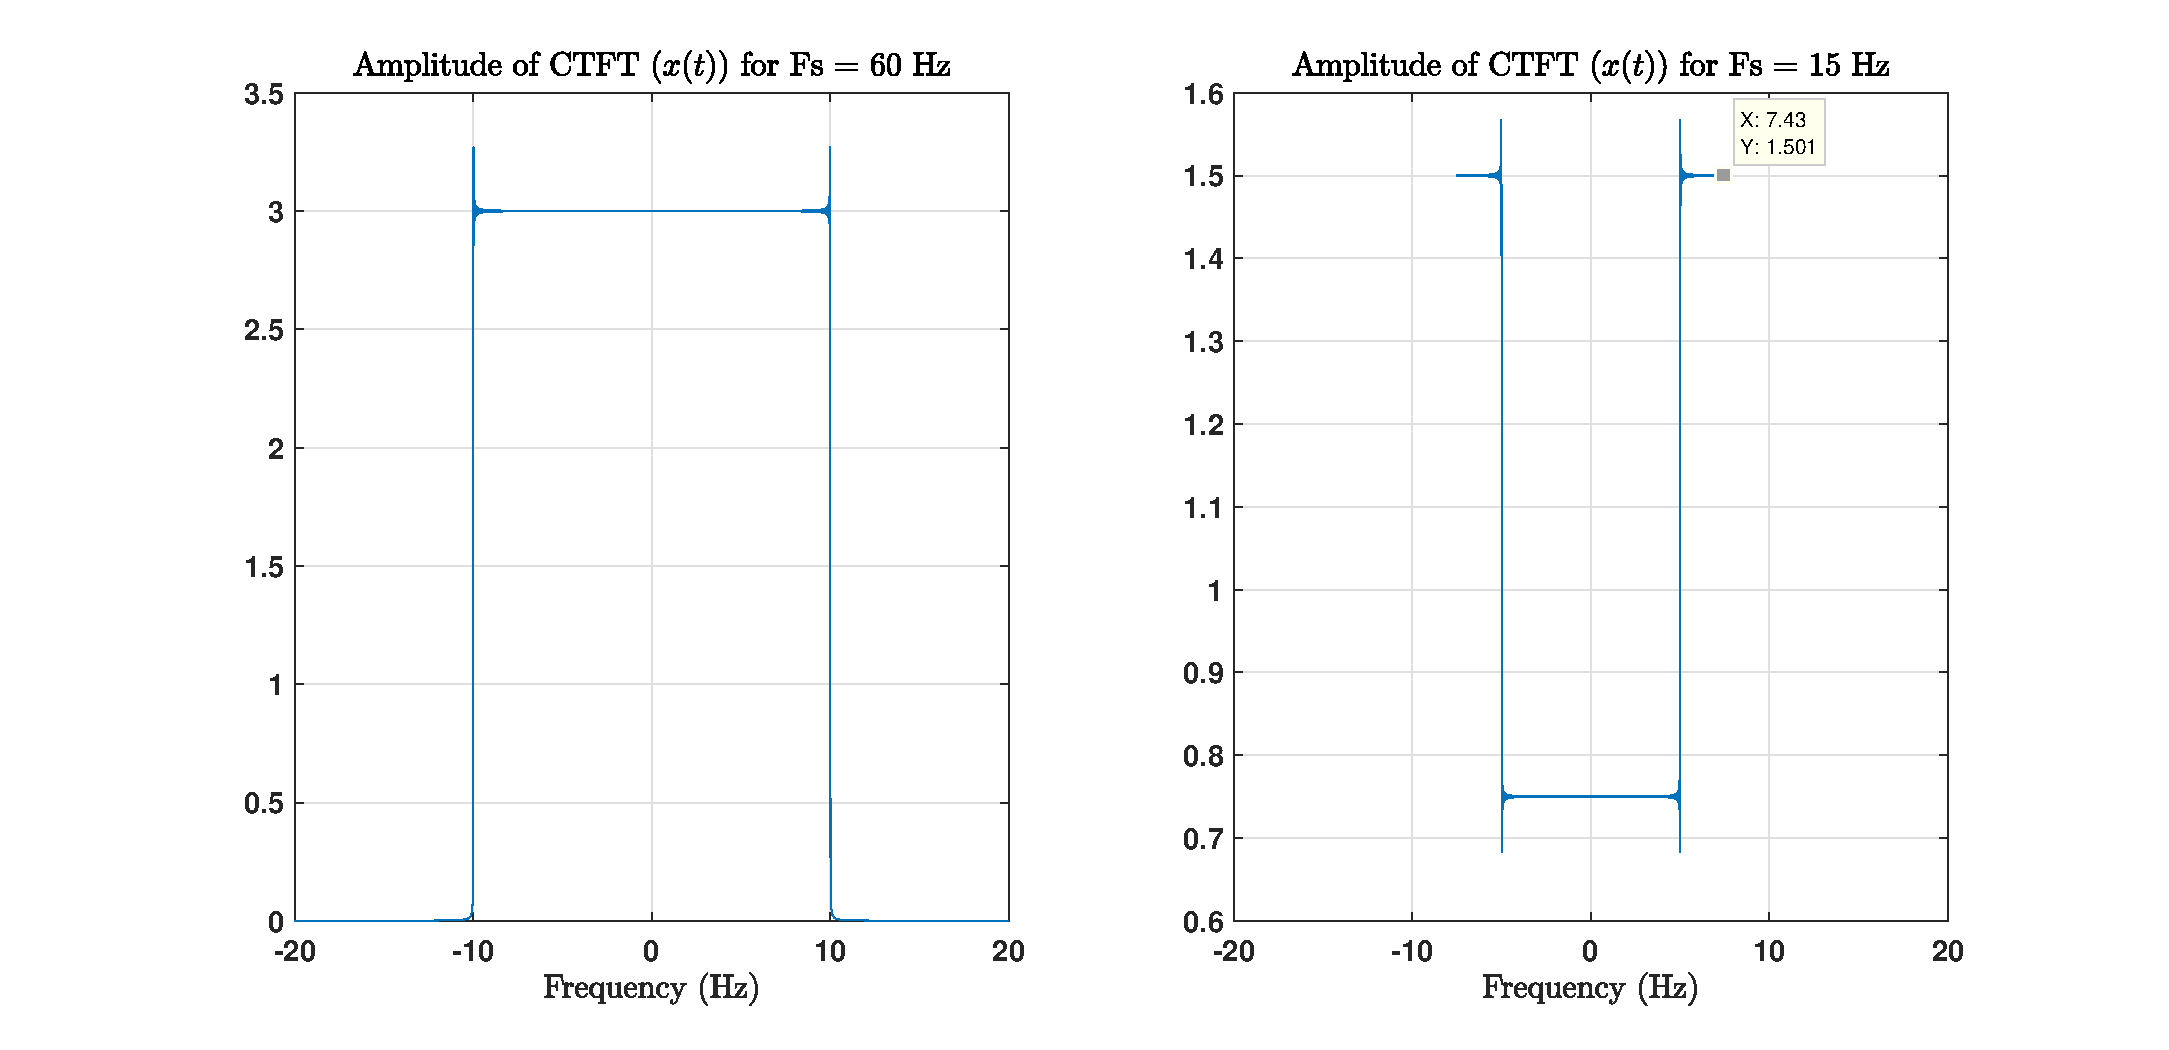
\includegraphics[scale = 0.45]{Figures/Sim_dowsampling_upsampling/CTFT_Amp_Sinc_B_10_Fs_60_15.eps}
\caption{Aliasing using $F_{s_{\text{ch}}} \, = \, 15$ Hz}
\label{fig:Sim_dowsampling_upsampling:CTFT_Amp_Sinc_B_10_Fs_60_15}
\end{figure}

\begin{itemize}
    \item the $F_s \, = \, 60$ Hz is just a reference, to compare aliased and unaliased spectrum
    
    \item For $F_s \, = \, 15$ Hz, my spectrum limit stop at 7.5 Hz and not at $B \, = \, 10$ Hz
    
    \begin{itemize}
    
        \item From my understanding of aliasing, I should get a spectrum of width $= \, B \, = \,10$ Hz, but distorted some how (addition of replica,from frequency exactly start the distortion,$\cdots$)
    
        \item This is because usually when simulating aliasing , I use fft(samples), where the samples are the downsampled giving a rate of 15 Hz (this is logic)
        
        \item \textit{But} (this is the important part) for frequency bins (which we as programmers generate): I generate it from $\displaystyle\frac{-F_s}{2} \, \rightarrow \, \displaystyle\frac{F_s}{2}$
        
        \item Doing so is fine when $F_s \,  > \, F_{\text{Nyquist}}$: In the left plot of \autoref{fig:Sim_dowsampling_upsampling:CTFT_Amp_Sinc_B_10_Fs_60_15} for $F_s \, = \, 60$ Hz, I did so and the spectrum is fine
        
        \item For the case of aliasing where $F_s \, = \, 15$ Hz, $\displaystyle\frac{-F_s}{2} \, \rightarrow \, \displaystyle\frac{F_s}{2} \, = \, -7.5 \, \rightarrow \, 7.5$ Hz
        
        
        \item However, I didn't in my life generate a frequency bins when taking an alias case, since in normal signal processing, we prevent aliasing and respect Nyquist sampling condition
        
        \item Clearly I need a more general way to implement aliasing in a correct way
        
    \end{itemize}
    
\end{itemize}

\newpage
\item I did some search, and I found this example from  matlab  documentation
    
    \begin{itemize}
        \item As motivation, when I search for examples to simulate aliasing over a full range of frequencies from $0 \, \rightarrow \, B$[Hz], it was the only convenient one
        
        \item Put the picture of the replicated spectrum when doing sampling, and say that my target is to simulate the idea that when sampling below Nyquist rate, distortion arise
        
        \item All other resources focus only on sin or cos (so only 1 active frequency component).\\
        
        \todo{aliasing resources} to cite the aliasing resource I have

    \end{itemize}
    
\item The example use discrete time approach, which is shown in \autoref{fig:Sim_dowsampling_upsampling:aliasing_demo_matlab_doc}
  
\begin{figure}[h]
\centering
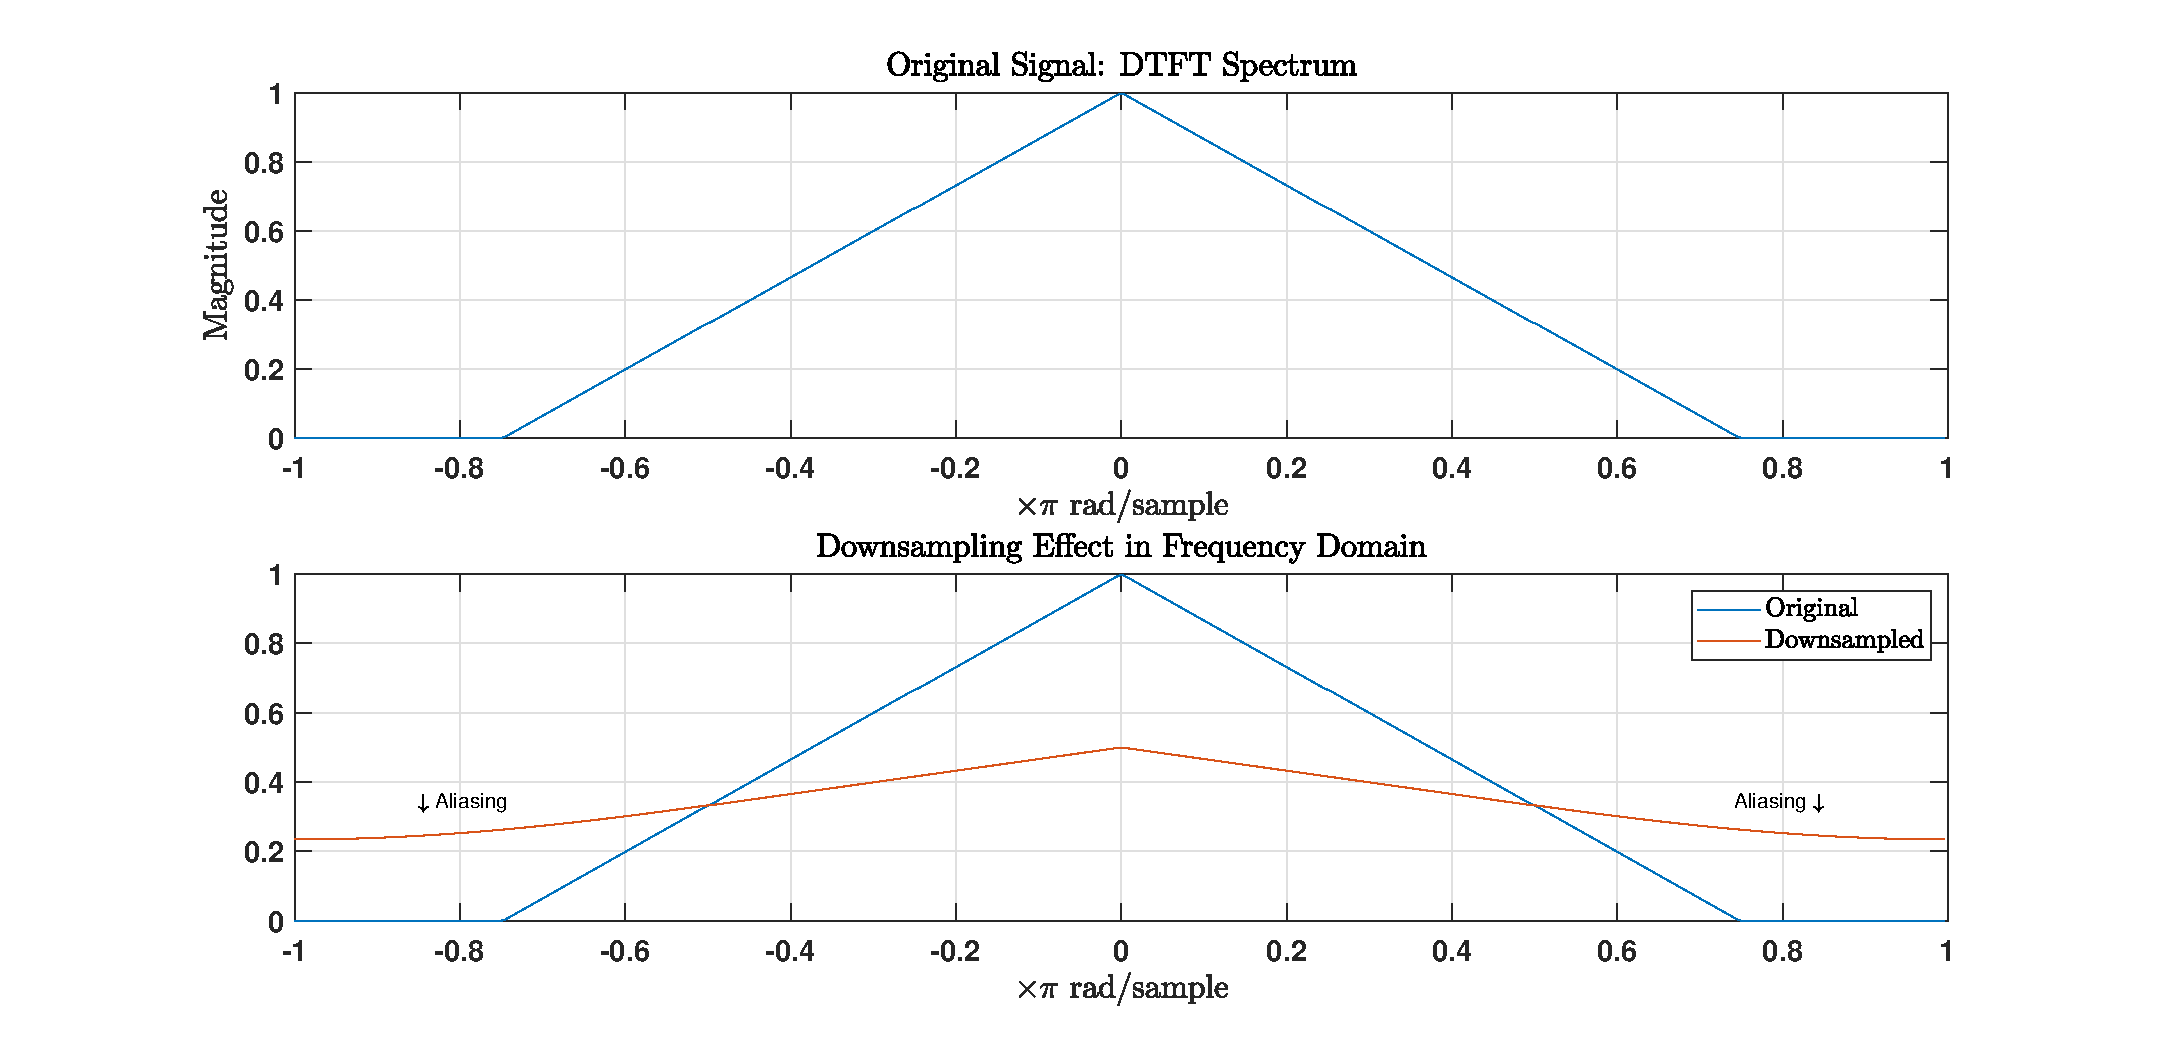
\includegraphics[scale = 0.45]{Figures/Sim_dowsampling_upsampling/aliasing_demo_matlab_doc}
\caption{Aliasing Example in discrete approach}
\label{fig:Sim_dowsampling_upsampling:aliasing_demo_matlab_doc}
\end{figure}  
    
\item \underline{Explanation of \autoref{fig:Sim_dowsampling_upsampling:aliasing_demo_matlab_doc}}    
    
    \begin{itemize}
    
    \item A \textit{discrete time bandlimited signal}   is generated, where the \textit{discrete bandwidth}  $= \, 0.75 \pi$ rad/cycle
    
    \item We do an integer downsampling operation of $D \, = \, 2$
    
    \item Recall that dowsampling doesn't necessary causes aliasing
    
    \item To know whether aliasing occurred or not, we test the following condition:
    
    \begin{equation}
    \text{Discrete Spectral support} \, < \, \displaystyle\frac{2 \pi}{D}
    \label{Eq:Aliasing_condition_discrete_freq_approach}
    \end{equation}
    
    \begin{itemize}
        \item If this is true, then dowsampling by $D \in \mathbb{N}$ won't cause aliasing
        
        \item If not, then aliasing occur
    \end{itemize}
    
    \item Back to the example, the \textit{Discrete Spectral support} contains \textit{positive discrete bandwidth} and the \textit{negative part} $\rightarrow$ \textit{Discrete Spectral support} $ \, = \, 0.75 \pi \, \times \, 2 \,  = \, 1.5 \, \pi$ rad/cycle
    
    \item Testing \autoref{Eq:Aliasing_condition_discrete_freq_approach} for $D \, = \, 2$, we get: $1.75 \pi > \displaystyle\frac{2 \pi}{D \, = \, 2} \, = \, \pi \rightarrow$ aliasing occur
    
    \begin{itemize}
        \item Spectral copies will overlap and get added
    \end{itemize}
    
    
    \item Although that aliasing is shown, \textit{but} there is no mention to any $F_s$ or ($T_s$): the example is simulated assuming that we are getting the discrete samples some how
    
    \begin{itemize}
        \item Recall that in our case (not just my case but also in real world), we express everything in Hz, seconds,$\cdots \leftrightarrow$ some meaningful units
        
        \item To get back from from radian/cycle $\rightarrow$  Hz, we use \cite{DSP_DimitrisManolakis}:
        
        \begin{equation}
                F \, [\text{Hz}] \, = \, \omega [\text{radian/cycle}] \, \times \, \left( \, \displaystyle\frac{F_s}{2 \pi} \, \, \right)
                \label{Eq:freq_conversion_rad_to_Hz}
        \end{equation}
        
        \item However, \autoref{Eq:freq_conversion_rad_to_Hz} is normally used when Nyquist theorem is respected $\leftrightarrow \, F_s \, > \, 2 \, \times f_{\text{max}}$
        
        \item But in our case, it is not
        
        \item So this give me a question, what $F_s$ should I use to obtain correctly a distorted spectrum according to \autoref{fig:Sim_dowsampling_upsampling:aliasing_illustration}
        
    \end{itemize}
    
        \item Put frequency conversion formula
        
        \item All the overlapping and the spectrum is inside $[-\pi \, , \, \pi]$, even when aliasing occurs
        
        \item Show the plot of a aliased sinc now, and compare it to the left plot of \autoref{fig:Sim_dowsampling_upsampling:CTFT_Amp_Sinc_B_10_Fs_60_15} 
        
    \end{itemize}

\item Applying concept in the example of \autoref{fig:Sim_dowsampling_upsampling:aliasing_demo_matlab_doc} to my case of sinc signal, where $B \, = \, 10$ Hz and $F_{s_{\text{ch}}} \, = \, 15$ Hz: 
        
\item Now when finishing from simulating in the discrete frequency domain, we need to move to the continuous frequency domain (that is $F$[Hz])

\begin{itemize}
    \item However, I have a problem which $F_s$ to use
     when doing the conversion
    
    
\end{itemize}


    
\end{itemize}



%*****************************************************
%*****************************************************
%*****************************************************